%%%%%%%%%%%%%%%%%%%%%%%%%%%%%%%%%%%%%%%%%%%%%%%%%%%%%%%%%%%%%%%%%
% MUW / EU-PEARL Presentation
% LaTeX Template
% Marta Bofill Roig and Pavla Krotka
% Vienna, 2022 February
%
% Based on MUW template:
% https://www.overleaf.com/latex/templates/medical-university-of-vienna-muw-presentation/dfhwmhfgkjck
%%%%%%%%%%%%%%%%%%%%%%%%%%%%%%%%%%%%%%%%%%%%%%%%%%%%%%%%%%%%%%%%%

\documentclass[10pt]{beamer} % Change 10pt to make fonts of a different size
\mode<presentation>

\usetheme{MUW}

%Colour themes
\usecolortheme{EUPEARL}
%\usecolortheme{MUW}

\setbeamertemplate{navigation symbols}{} 
\setbeamertemplate{caption}[numbered]
\usepackage[english]{babel}
\usepackage[utf8x]{inputenc}

%%%%%%%%%%%%%%%%%%%%%%%%%%%%%%%%%%%%%%%%%%%%%%%%%%%%%%%%%%%%%%%%%
%% FONTS
%\usefonttheme{serif}  % Uncomment for all serif fonts
%% Comment the following two lines for sans serif fonts in titles
%\setbeamerfont{frametitle}{family=\fontfamily{cmr}}
%\setbeamerfont{title}{family=\fontfamily{cmr}}
\usepackage{helvet}
\usefonttheme{serif}
%%%%%%%%%%%%%%%%%%%%%%%%%%%%%%%%%%%%%%%%%%%%%%%%%%%%%%%%%%%%%%%%%


%%%%%%%%%%%%%%%%%%%%%%%%%%%%%%%%%%%%%%%%%%%%%%%%%%%%%%%%%%%%%%%%%
%% Presentation Info
\title[Your Short Title]{Main Title}
\author[email]{Author}
\institute{Affiliation}
\date{\today}
%%%%%%%%%%%%%%%%%%%%%%%%%%%%%%%%%%%%%%%%%%%%%%%%%%%%%%%%%%%%%%%%%


%%%%%%%%%%%%%%%%%%%%%%%%%%%%%%%%%%%%%%%%%%%%%%%%%%%%%%%%%%%%%%%%%
%% FOOTLINE
%% Comment/Uncomment the following blocks to modify the footline
%% content in the body slides. 

%MUW
%% Option A: Title and institute
%\footlineA
%% Option B: Author and institute
%\footlineB
%% Option C: Title, Author and institute
%\footlineC
%% Option MUW modified 1 - without logo
%\footlineMUWsmall
%% Option MUW modified 2 - with logo
%\footlineMUWm

%% Option EU-PEARL
\footlineEUPEARL
%% Option EU-PEARL modified - small logo and 3 columns
%\footlineEUPEARLsmall

%%%%%%%%%%%%%%%%%%%%%%%%%%%%%%%%%%%%%%%%%%%%%%%%%%%%%%%%%%%%%%%%%

\begin{document}

%%%%%%%%%%%%%%%%%%%%%%%%%%%%%%%%%%%%%%%%%%%%%%%%%%%%%%%%%%%%%%%%%
% Use this block for a blue MUW title slide with modified footline
% {\titlepageBlue
% \begin{frame}
%   \titlepage
% \end{frame}
% }

% Use this block for a blue EU-PEARL title slide with modified footline
{\titlepageBlueEUP
\begin{frame}
  \titlepage
\end{frame}
}

%%%%%%%%%%%%%%%%%%%%%%%%%%%%%%%%%%%%%%%%%%%%%%%%%%%%%%%%%%%%%%%%%
% Use this block for a white MUW title slide with modified footline
% {\titlepageWhite
% \begin{frame}
%   \titlepage
% \end{frame}
% }

% Use this block for a white EU-PEARL title slide with modified footline
{\titlepageWhiteEUP
\begin{frame}
  \titlepage
\end{frame}
}

%%%%%%%%%%%%%%%%%%%%%%%%%%%%%%%%%%%%%%%%%%%%%%%%%%%%%%%%%%%%%%%%%
% Comment/Uncomment these lines for an automatically generated outline.
\begin{frame}{Outline}
  \tableofcontents
\end{frame}


\addtocounter{framenumber}{-1} %To control the number in which numbering begins

%%%%%%%%%%%%%%%%%%%%%%%%%%%%%%%%%%%%%%%%%%%%%%%%%%%%%%%%%%%%%%%%%
\section{Introduction}
\begin{frame}{Introduction}
\begin{itemize}
  \item Your introduction goes here!
  \item Use \texttt{itemize} to organize your main points.
  \begin{itemize}
  	\item up to 3 text levels with \texttt{itemize}
	\begin{itemize}
  	  	\item Indents increase level by level, font size decreases
		\begin{description}[abc]  % for indentation of length of abc
  			\item[$\bullet$] Should you require more levels, use \texttt{description} instead of \texttt{itemize}.
        	\begin{description}[abc]  % for indentation of length of abc
  				\item[$\bullet$] Note: Please try not to write too much copy onto your slides.
			\end{description}
		\end{description}
	\end{itemize}
  \end{itemize}
\end{itemize}

\end{frame}

%%%%%%%%%%%%%%%%%%%%%%%%%%%%%%%%%%%%%%%%%%%%%%%%%%%%%%%%%%%%%%%%%
\section{Section 1}
{\sectionheaderWhite %Enclose the frame with {} and add this command for white background in section header
\begin{frame}{Section Header 1}{Version - white background}
\end{frame}
}

%%%%%%%%%%%%%%%%%%%%%%%%%%%%%%%%%%%%%%%%%%%%%%%%%%%%%%%%%%%%%%%%%
\section{Section 2}
{\sectionheaderSkin %Enclose the frame with {} and add this command for skin background in section header
\begin{frame}{Section Header 2}{Version - backgroundcolour skin}
\end{frame}
}

%%%%%%%%%%%%%%%%%%%%%%%%%%%%%%%%%%%%%%%%%%%%%%%%%%%%%%%%%%%%%%%%%
\section{Section 3}
{\sectionheaderGreen %Enclose the frame with {} and add this command for green background in section header
\begin{frame}{Section Header 3}{Version - backgroundcolour green}
\end{frame}
}

%%%%%%%%%%%%%%%%%%%%%%%%%%%%%%%%%%%%%%%%%%%%%%%%%%%%%%%%%%%%%%%%%
\section{Content}
% Slide with black Background
{\blackSlide %Enclose the frame with {} and add this command for black background in frame
\begin{frame}{Title and Content - Black}
\begin{columns}
  \begin{column}{0.3\textwidth}
    \begin{center}
     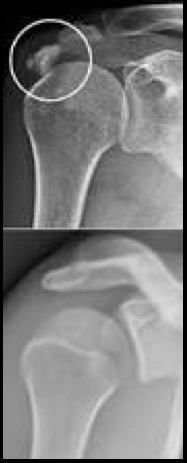
\includegraphics[width=0.8\textwidth]{Images/xray.png}
     \end{center}
  \end{column}
  \begin{column}{0.7\textwidth}  %%<--- here
    \begin{itemize}
	  \item Especially for pictures like x-ray
	  \item Enter explanation text - e.g. what can be seen in the picture
	\end{itemize}
  \end{column}
\end{columns}

\end{frame}
}


%%%%%%%%%%%%%%%%%%%%%%%%%%%%%%%%%%%%%%%%%%%%%%%%%%%%%%%%%%%%%%%%%
\begin{frame}{Title, subtitle and content}{Enter subtitle here}
Enter text, charts, pictures, … here
\end{frame}

%%%%%%%%%%%%%%%%%%%%%%%%%%%%%%%%%%%%%%%%%%%%%%%%%%%%%%%%%%%%%%%%%
\section{Figures}
\begin{frame}{Figures}

\begin{itemize}
  \item You can upload a figure (JPEG, PNG or PDF) using the files menu. 
  \item To include it in your document, use the \texttt{includegraphics} command (see the comment below in the source code).
\end{itemize}

% Commands to include a figure:
\begin{figure}
  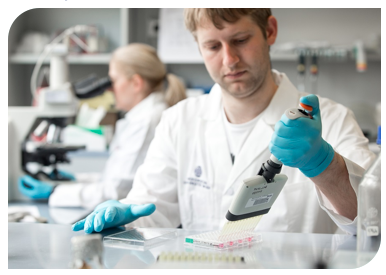
\includegraphics[width=0.5\textwidth]{Images/image.png}
  \caption{\label{fig:your-figure}Caption goes here.}
\end{figure}

\end{frame}  

%%%%%%%%%%%%%%%%%%%%%%%%%%%%%%%%%%%%%%%%%%%%%%%%%%%%%%%%%%%%%%%%%
\begin{frame}{Blocks}

\begin{block}{Block}
Some examples of commonly used commands and features are included, to help you get started.
\end{block}

\begin{exampleblock}{Example Block}
Some examples of commonly used commands and features are included, to help you get started.
\end{exampleblock}

\begin{alertblock}{Alert Block}
Some examples of commonly used commands and features are included, to help you get started.
\end{alertblock}

\end{frame}

%%%%%%%%%%%%%%%%%%%%%%%%%%%%%%%%%%%%%%%%%%%%%%%%%%%%%%%%%%%%%%%%%
\section{Some \LaTeX{} Examples}
\subsection{Tables}

\begin{frame}{Tables}{Tables}

\begin{table}
\centering
\begin{tabular}{l|r}
Item & Quantity \\\hline
Widgets & 42 \\
Gadgets & 13
\end{tabular}
\caption{\label{tab:widgets}An example table.}
\end{table}

\end{frame}

%%%%%%%%%%%%%%%%%%%%%%%%%%%%%%%%%%%%%%%%%%%%%%%%%%%%%%%%%%%%%%%%%
\subsection{Mathematics}

\begin{frame}{Readable Mathematics}

Let $X_1, X_2, \ldots, X_n$ be a sequence of independent and identically distributed random variables with $\text{E}[X_i] = \mu$ and $\text{Var}[X_i] = \sigma^2 < \infty$, and let
$$S_n = \frac{X_1 + X_2 + \cdots + X_n}{n}
      = \frac{1}{n}\sum_{i}^{n} X_i$$
denote their mean. Then as $n$ approaches infinity, the random variables $\sqrt{n}(S_n - \mu)$ converge in distribution to a normal $\mathcal{N}(0, \sigma^2)$.

\end{frame}


\end{document}
